\documentclass[11pt]{exam}
\usepackage[phy]{template-for-exam}
\usepackage{tikz}
\usetikzlibrary{arrows.meta}

\title{Equation Sheet - Fall Final Exam}
\author{Rohrbach}
\date{\today}

\begin{document}
\maketitle


\hrule
\section*{Science \& Measurement}

  \begin{minipage}{.7\textwidth}
    \begin{center}
      \begin{align*}
        \text{\% error} &= \frac{\left| \text{measured} - \text{expected} \right|}{\text{expected}} \times 100
      \end{align*}
    \end{center}
  \end{minipage}
  %
  \begin{minipage}{.25\textwidth}
    \begin{tabular}{ccc}
      \hline
      \multicolumn{3}{c}{Metric Prefixes}                 \\
      \hline
      \SI{}{\kilo\relax}  & kilo-          & \SI{e3}{}  \\
            --            & (\textit{base})& $10^0$     \\
      \SI{}{\centi\relax} & centi-         & \SI{e-2}{} \\
      \SI{}{\milli\relax} & milli-         & \SI{e-3}{} \\
      \SI{}{\micro\relax} & micro-         & \SI{e-6}{} \\
      \SI{}{\nano\relax}  & nano-          & \SI{e-9}{} \\
      \hline
    \end{tabular}
    \vspace*{1em}
  \end{minipage}





\hrule
\section*{Motion \& Kinematics}

  \subsection*{Constant Velocity \& Acceleration}

      \begin{align*}
          v       &= \frac{d}{t}
        & a       &= \frac{\Delta v}{t}
        &\Delta v &= v_f - v_i
      \end{align*}



  \subsection*{Constant Acceleration}

    \begin{align*}
        v_f   &=  v_i + at 
      & d     &=  v_i t + \frac{1}{2} a t^2
      & v_f^2 &=  v_i^2 + 2 a d \\
      \omit\rlap{\it\footnotesize ``Old Faithful''} &&
      \omit\rlap{\it\footnotesize ``The Big Chalupa''} &&
      \omit\rlap{\it\footnotesize ``Ain't Got No Time''}
    \end{align*}

  \subsection*{Vector Equations}

    \begin{minipage}[b]{.7\linewidth}
      \begin{align*}
        \theta &= \tan^{-1} \left( v_y / v_x \right) &
        v_x^2 + v_y^2 &= v_R^2
      \end{align*}

      \vspace{-2em}

      \begin{align*}
        v_x    &= v_R \cos \left( \theta \right) &
        v_y    &= v_R \sin \left( \theta \right)
      \end{align*}
    \end{minipage}
    %
    \begin{minipage}{.28\linewidth}
      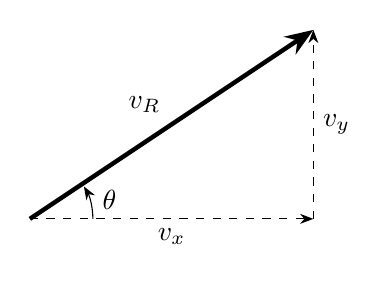
\begin{tikzpicture}[
          component/.append style={
            dashed,
            -{Stealth}
          },
          resultant/.append style={
            ultra thick,
            -{Stealth}
          },
          scale=0.8
      ]
        \draw[resultant] 
                  (0,0) -- (4.5,3) 
                    node[midway,anchor=south east]{\bf $v_R$};
        \draw[component] 
                  (0,0) 
                  -- (4.5,0) 
                    node[midway,anchor=north]{$v_x$} ;
        \draw[component] 
                  (4.5,0)
                  -- (4.5,3) 
                    node[midway, anchor=west]{$v_y$} ;
        \draw[-Stealth] (1,0) node[anchor=south west]{$\theta$}
                  arc[
                    start angle = 0,
                    end angle = 31, 
                    radius = 1
                  ];
      \end{tikzpicture}
    \end{minipage}

    
\hrule
\section*{Forces}

  \begin{align*}
    F_{NET} &=  ma
  & F_{NET} &=  \pm F_1 \pm F_2 \pm \cdots
  & F_G     &=  mg
  & g       &= \SI{9.8}{\meter\per\second^2}
\end{align*}


\hrule
\section*{Circular Motion \& Gravity}

    
    \begin{align*}
        T     &=  \frac{t}{\text{\#rot}}
      & v_T   &=  \frac{2\pi r}{T}
      & v_T   &=  r\omega
      & \omega&= \frac{\text{\#rot}}{t}\times 2\pi
      & F_C   &= \frac{mv_T^2}{r}
    \end{align*}

  \begin{align*}
    F_G &= \frac{Gm_1m_2}{d^2} 
    & G &= \SI{6.67e-11}{\newton\meter^2\per\kilo\gram^2}
  \end{align*}

\end{document}